\documentclass[twocolumn]{article}

\usepackage{arxiv}
\usepackage{amsmath,amssymb}
\usepackage{graphicx}
\usepackage{hyperref}
\usepackage{booktabs}
\usepackage[numbers]{natbib}
\usepackage{authblk}

\renewcommand{\headeright}{}
\renewcommand{\undertitle}{}

\title{PrivateBoost: Privacy-Preserving Federated Gradient Boosting for Cross-Device Medical Data}

\author[1,2]{Bernhard Specht\thanks{Corresponding author: \texttt{bernhard.specht@myelinz.com}}}
\author[1]{Samaher Garbaya}
\author[3]{Orhan Ermis}
\author[4]{Reinhard Schneider}
\author[5]{Ricardo Chavarriaga}
\author[3]{Djamel Khadraoui}
\author[1,6]{Zied Tayeb}

\affil[1]{MyelinZ, Manchester, UK / San Francisco, USA / Leuven, Belgium /Luxembourg}
\affil[2]{University of Luxembourg, Esch-sur-Alzette, Luxembourg}
\affil[3]{Luxembourg Institute of Science and Technology (LIST), Esch-sur-Alzette, Luxembourg}
\affil[4]{Luxembourg Centre for Systems Biomedicine (LCSB), Esch-sur-Alzette, Luxembourg}
\affil[5]{ZHAW Zurich University of Applied Sciences, Winterthur, Switzerland}
\affil[6]{University of Lincoln, Lincoln, United Kingdom}

\date{}

\begin{document}

\twocolumn[
  \maketitle
  \begin{@twocolumnfalse}
  \begin{abstract}
Cross-device medical federated learning where individual patients participate directly rather than institutions poses a unique challenge: each client holds only a few samples, often just one (e.g., a single diagnostic record), leaving insufficient local data for gradient computation. Existing approaches, such as Secure Aggregation, require client-to-client coordination impractical for intermittently available mobile devices, while homomorphic encryption-based alternatives introduce sophisticated key management and coordination requirements ill-suited to dynamic cross-device deployments. We present \textit{privateboost}, a federated XGBoost system that addresses this setting through m-of-n Shamir secret sharing with commitment-based anonymous aggregation. Clients distribute shares to a fixed set of shareholders requiring no client-to-client communication and the aggregator reconstructs only aggregate gradient sums via Lagrange interpolation, never observing individual values or client identities. We evaluate on UCI medical datasets, demonstrating 98\% split gain retention relative to centralized XGBoost and accuracy resilient to up to 80\% client dropout.
  \end{abstract}
  \vspace{1em}
  \end{@twocolumnfalse}
]

\section{Introduction}

Federated learning enables machine learning on distributed data without centralizing raw samples~\cite{mcmahan2017}. However, much existing work focuses on a \textit{cross-silo} setting where each client (typically an organization) holds multiple data samples and can perform local training~\cite{kairouz2021}. Popular frameworks such as Flower~\cite{beutel2020flower} and NVIDIA FLARE~\cite{roth2022nvidia} support both settings but are primarily evaluated in cross-silo or simulated deployments.

In medical settings, ``federated learning'' typically means hospitals or research institutions each manage patient cohorts~\cite{rieke2020,sheller2020}, with the institution serving as a trusted aggregation point for its patients' data. True \textit{cross-device} medical federated learning, where individual patients control their own records without institutional intermediaries, remains largely unexplored. Cross-device settings have been studied for applications like mobile keyboard prediction~\cite{hard2018}, but medical applications present unique challenges.

First, \textit{extreme non-IID data}: each client holds only a few samples, often just one. A patient participating in a federated study may contribute only their single health record. There are no local batches large enough for meaningful gradient computation; each participant is effectively a single data point. Second, tree-based methods like XGBoost~\cite{chen2016} require global statistics (gradient histograms across all samples) to find optimal split points. Without local batches large enough for meaningful statistics or secure aggregation, clients cannot contribute to these histograms without revealing their individual values.

Existing privacy-preserving approaches face practical barriers in this setting. SecAgg~\cite{bonawitz2017} requires client-to-client coordination for pairwise key agreement, which is problematic when clients are intermittently online mobile devices. Additionally, homomorphic encryption-based solutions can serve as alternative secure aggregation mechanisms, namely multi-key and multi-party homomorphic encryption schemes~\cite{wu2025smhe,cheon2025mphe}. However, such mechanisms require sophisticated key management procedures, including distributed key generation, key switching, and evaluation key distribution. Therefore, homomorphic encryption-based schemes introduce additional protocol complexity and coordination requirements, which may be difficult to satisfy in highly dynamic cross-device deployments with frequently joining and leaving clients.

We present \textit{privateboost}, a privacy-preserving federated XGBoost system designed for the one-sample-per-client setting:

\begin{enumerate}
  \item A protocol using m-of-n Shamir secret sharing with commitment-based client anonymity
  \item A three-party architecture (clients $\to$ shareholders $\to$ aggregator) requiring no client-to-client communication
  \item Privacy guarantees: raw data never leaves the client; shareholders see only shares; the aggregator sees only aggregate sums. Hence, under the non-collusion assumption, where fewer than $m$ shareholders collude, individual gradients shared by clients are information-theoretically secure
  \item Empirical validation on medical datasets demonstrating 98\% split gain retention with dropout resilience
\end{enumerate}

\section{Related Work}

\subsection{Secure Aggregation}

SecAgg~\cite{bonawitz2017} enables a server to compute sums of client updates without learning individual values. The protocol uses pairwise masking: each pair of clients agrees on a random mask via Diffie-Hellman key exchange, and these masks cancel when the server sums all contributions. This requires $O(n)$ pairwise key agreements per client and coordination to handle dropouts. Subsequent work has reduced communication to polylogarithmic overhead~\cite{bell2020}, but the protocols still rely on structured communication patterns between clients.

Our approach uses a star topology where clients distribute shares to a fixed set of shareholders without any client-to-client communication. This is better suited to cross-device settings where clients are intermittently available.

\subsection{Federated Gradient Boosting}

Gradient boosting~\cite{friedman2001} builds ensembles of weak learners. LightGBM~\cite{ke2017} uses histogram-based split finding for efficiency; XGBoost~\cite{chen2016} supports both exact and approximate histogram methods.

SecureBoost~\cite{cheng2021} addresses federated XGBoost in the \textit{vertical} federated learning setting, where different parties hold different features for the same samples. This assumes institutional participants with aligned datasets. Federated Forest~\cite{liu2020fedforest} similarly targets cross-silo settings with multiple samples per participant. Recent work has extended secret sharing to vertical federated XGBoost~\cite{xie2022fedxgb}, and FedTree~\cite{li2023fedtree} provides a comprehensive system supporting both horizontal and vertical settings with configurable privacy techniques.

For \textit{horizontal} federated learning, SimFL~\cite{li2020simfl} uses locality-sensitive hashing (LSH) to share similarity information between parties. However, SimFL's design assumes each party holds many samples: each party builds trees using only its local instances, weighted by gradients from similar samples at other parties. This fundamentally precludes the one-sample-per-client setting. Additionally, LSH-based approaches have weaker privacy guarantees than cryptographic methods: parties learn which samples are similar across institutions, which could enable inference attacks on sensitive medical data.

Differential privacy has also been applied to gradient boosting~\cite{li2020ppgbdt} in centralized settings, but these approaches assume access to the full dataset and do not address the federated or cross-device setting.

Table~\ref{tab:comparison} summarizes the key properties of existing federated tree-learning approaches. Our work addresses the orthogonal \textit{horizontal} federated setting with extreme non-IID: one sample per client, providing information-theoretic security via secret sharing rather than the computational security of LSH-based approaches.

\begin{table*}[t]
  \centering
  \caption{Comparison of federated tree-learning approaches. HE = homomorphic encryption, SA = secure aggregation, DP = differential privacy, LSH = locality-sensitive hashing, SS = secret sharing, C2C = client-to-client, X-device = cross-device.}
  \label{tab:comparison}
  \footnotesize
  \begin{tabular}{@{}lllllcc@{}}
    \toprule
    \textbf{Method} & \textbf{Setting} & \textbf{Privacy} & \textbf{Security} & \textbf{Min.\ Samples} & \textbf{No C2C} & \textbf{X-device} \\
    \midrule
    SecureBoost~\cite{cheng2021}         & Vertical     & HE (Paillier)        & Computational      & Many       & \checkmark & -- \\
    Fed.\ Forest~\cite{liu2020fedforest} & Vertical     & Encoding + encryption & Computational      & Many       & \checkmark & -- \\
    SimFL~\cite{li2020simfl}             & Horizontal   & LSH                  & Computational      & Many       & --         & -- \\
    Xie et al.~\cite{xie2022fedxgb}     & Vertical     & Secret sharing       & Info-theoretic     & Many       & --         & -- \\
    FedTree~\cite{li2023fedtree}         & Both         & HE / SA / DP         & Configurable       & Many       & \checkmark & -- \\
    \textit{privateboost} (ours)         & Horizontal   & Shamir SS            & Info-theoretic     & \textbf{1} & \checkmark & \checkmark \\
    \bottomrule
  \end{tabular}
\end{table*}

\subsection{Secret Sharing in Machine Learning}

Shamir secret sharing~\cite{shamir1979} is a foundational primitive for multi-party computation (MPC)~\cite{benor1988}. Verifiable extensions~\cite{gennaro1998} enable detection of malicious behavior. These techniques have been applied in MPC frameworks for machine learning inference, but not extensively explored for federated training.

The key property we exploit is \textit{additive homomorphism}: the sum of shares equals shares of the sum, enabling aggregation without reconstruction of individual values.

\section{Protocol}

\subsection{Background: Histogram-Based Split Finding}

XGBoost~\cite{chen2016} builds decision trees by greedily selecting splits that maximize a gain function. For each node, the algorithm considers every feature and every possible split threshold. To make this tractable, histogram-based methods discretize continuous features into $B$ bins and compute gradient statistics per bin.

Each sample $i$ contributes a gradient $g_i = \partial L / \partial \hat{y}_i$ and Hessian $h_i = \partial^2 L / \partial \hat{y}_i^2$ based on the current prediction $\hat{y}_i$ and true label $y_i$. For a candidate split that partitions samples into left ($L$) and right ($R$) sets, the gain is:

\begin{equation}
  \text{Gain} = \frac{1}{2} \left[ \frac{G_L^2}{H_L + \lambda} + \frac{G_R^2}{H_R + \lambda} - \frac{(G_L + G_R)^2}{H_L + H_R + \lambda} \right]
\end{equation}

where $G_L = \sum_{i \in L} g_i$, $H_L = \sum_{i \in L} h_i$, and $\lambda$ is a regularization parameter. The key insight is that split finding requires only \textit{aggregate} gradient sums per bin, not individual gradients. Our protocol computes these sums without revealing individual contributions.

\subsection{System Model}

We consider $c$ clients, each holding a single labeled sample $(x_i, y_i)$. A set of $n$ \textit{shareholders} (e.g., $n = 3$) act as intermediate aggregation points. A single \textit{aggregator} coordinates the training process. Figure~\ref{fig:architecture} illustrates the overall system architecture.

\begin{figure*}[t]
  \centering
  
\includegraphics[width=0.9\textwidth]{figures/architecture.png}
  \caption{System architecture. Clients distribute Shamir shares to all shareholders. Shareholders sum received shares and forward partial sums to the aggregator, which reconstructs aggregate statistics ($\Sigma x$, $\Sigma x^2$ for binning) and gradient sums ($\Sigma G$, $\Sigma H$ for splits). The aggregator broadcasts bin configurations and split decisions back to clients.}
  \label{fig:architecture}
\end{figure*}

The adversarial assumptions underlying this architecture are detailed in the threat model (Section~\ref{sec:threat-model}).

\subsection{Building Blocks}

\textbf{Shamir Secret Sharing.} To share a secret value $s$, sample a random polynomial $f(x)$ of degree $m-1$ with $f(0) = s$. Distribute shares $(i, f(i))$ for $i = 1, \ldots, n$ to $n$ shareholders. Any $m$ shares can reconstruct $s$ via Lagrange interpolation; fewer than $m$ shares reveal nothing about $s$.

\textbf{Additive Homomorphism.} For shares of values $a$ and $b$, the sum of shares equals shares of $(a + b)$. This allows shareholders to sum their received shares without learning individual values, and the aggregator reconstructs only the sum.

\textbf{Commitments.} Each client generates a commitment $c = H(\text{round} \| \text{client\_id} \| \text{nonce})$ using a fresh nonce per round. Shareholders only sum shares that have matching commitment hashes, ensuring consistent aggregation: if a client's share reaches some shareholders but not others, those shares are excluded rather than causing corrupted reconstruction. The aggregator sees only commitment hashes, not client identifiers.

\subsection{Protocol Flow}

The protocol has two phases: a one-time statistics phase to define histogram bins, followed by repeated gradient phases to build trees.

\textbf{Phase 1: Statistics.} Before training, the aggregator needs feature statistics to define histogram bin edges. Each client $i$ creates Shamir shares of their feature values $x_{i,f}$ and squared values $x_{i,f}^2$ for each feature $f$, along with a commitment. Clients send shares to shareholders. The aggregator requests sums from shareholders, reconstructs $\sum x$ and $\sum x^2$, computes per-feature mean $\mu$ and variance $\sigma^2$, and defines $B$ equal-width bins spanning $\mu \pm 3\sigma$. The aggregator broadcasts bin edges to all clients.

\textbf{Phase 2: Gradient Rounds.} For each tree and each depth level, the aggregator needs gradient sums per (feature, bin) combination. Each client $i$:

\begin{enumerate}
  \item Computes their gradient $g_i$ and Hessian $h_i$ from current ensemble prediction
  \item For each feature $f$, determines which bin $b$ their value $x_{i,f}$ falls into
  \item Creates Shamir shares of $(g_i, h_i)$ with a fresh commitment
  \item Sends shares to shareholders, tagged with $(f, b, \text{commitment})$
\end{enumerate}

Shareholders accumulate shares grouped by (feature, bin, commitment). When the aggregator requests sums for a set of commitments, each shareholder returns summed shares per (feature, bin). The aggregator reconstructs gradient sums $G_{f,b} = \sum g_i$ and $H_{f,b} = \sum h_i$ for each bin, evaluates the gain formula for each possible split, selects the best split, and broadcasts the decision (feature, threshold) to clients. Clients update their node assignments, and the process repeats for the next depth level.

After reaching maximum depth, leaf values are computed from gradient sums and the tree is added to the ensemble. The entire gradient phase repeats for each tree.

\section{Security Analysis}

\subsection{Threat Model}
\label{sec:threat-model}

We assume an honest-but-curious (semi-honest) adversary model: all parties follow the protocol correctly but may attempt to learn additional information from their observations.

\textbf{Shareholders.} At most $m-1$ out of $n$ shareholders may collude for an $m$-of-$n$ threshold scheme. The collusion threshold is configurable: increasing from 2-of-3 to 3-of-5 or higher provides stronger guarantees while maintaining dropout tolerance. Shareholders enforce a minimum-client threshold: they refuse to release aggregate sums if fewer than a configurable minimum number of clients contributed shares, preventing reconstruction from insufficiently anonymized aggregates. Crucially, shareholders do not collude with the aggregator; any such collusion would undermine the separation between share-level and aggregate-level views that the protocol relies on.

\textbf{Aggregator.} A single aggregator coordinates the protocol. It follows the protocol honestly but may attempt to learn individual values from the aggregates it reconstructs. It does not have access to raw shares or client identifiers.

\textbf{Clients.} Clients are assumed honest-but-curious. The protocol does not include cryptographic verification of individual contributions; defenses against malicious clients are discussed in Section~\ref{sec:limitations}.

\subsection{Privacy Guarantees}

\textbf{Clients} hold their raw feature values and labels locally. Each client submits Shamir shares along with a pseudonymous client identifier (to prevent duplicate submissions) to shareholders. This identifier is linked to an account but does not reveal the client's real identity. Since shares are information-theoretically secure, no single shareholder can learn anything about the original values.

\textbf{Shareholders} receive shares tagged with client identifiers and commitment hashes. They use identifiers to prevent duplicate submissions but do not forward them to the aggregator. Under the collusion threshold defined in the threat model, shareholders cannot reconstruct individual values. Shareholders sum shares for requested commitments and return only these aggregated sums.

\textbf{The aggregator} receives summed shares from shareholders and reconstructs aggregate gradient sums via Lagrange interpolation. Crucially, it never sees client identifiers, only opaque commitment hashes. It learns split thresholds (necessary for prediction) and gradient sums per bin. It learns how many clients fall into each tree branch, but not which specific clients.

\subsection{Communication and Computation Cost}

Let $c$ denote the number of clients, $F$ the number of features, $B$ the number of bins, $n$ the number of shareholders, $m$ the reconstruction threshold, $T$ the number of trees, and $d$ the maximum tree depth.

\textbf{Communication.} In the one-time statistics phase, each client creates Shamir shares of $2F$ values ($x_{i,f}$ and $x_{i,f}^2$) and distributes them to $n$ shareholders, yielding $O(Fcn)$ total shares. In each gradient round (one depth level of one tree), each client shares $2F$ gradient values ($g_i$ and $h_i$ per feature), producing $O(Fcn)$ shares per round. Over $T$ trees at depth $d$, total client-to-shareholder communication is $O(TdFcn)$. Each shareholder returns $O(FB)$ partial sums to the aggregator per round, giving $O(TdFBn)$ shareholder-to-aggregator communication. The aggregator broadcasts a single split decision per round.

\textbf{Computation.} Creating a Shamir share requires evaluating a degree-$(m{-}1)$ polynomial at $n$ points, costing $O(nm)$ per value. Each client thus performs $O(Fnm)$ work per gradient round, or $O(TdFnm)$ total. Shareholders sum $O(c)$ shares per (feature, bin) bucket. The aggregator performs Lagrange interpolation over $m$ points for each of the $O(FB)$ aggregate values per round, costing $O(TdFBm^2)$ total. Split finding adds $O(TdFB)$.

\textbf{Scalability in $n$.} Communication grows linearly in $n$ (more shares to distribute and collect). Computation for sharing grows as $O(nm)$, and reconstruction depends only on $m$, not $n$. Increasing $n$ while keeping $m$ fixed improves fault tolerance (more shareholders can drop out) without affecting reconstruction cost. Increasing $m$ strengthens the collusion threshold at the cost of higher-degree polynomials for sharing and $O(m^2)$ Lagrange reconstruction.

\subsection{Limitations}
\label{sec:limitations}

\textbf{Branch counts.} The aggregator learns client counts per tree branch. For branches with very few clients, this narrows the anonymity set. Combined with auxiliary information, this could enable inference attacks. This motivates k-anonymous tree constraints (Section~\ref{sec:k-anonymous}).

\textbf{Shareholder path visibility.} Shareholders observe which bin each client submits gradients to, revealing individual tree paths. This can be addressed using the path hiding technique described in Section~\ref{sec:path-hiding}: clients submit shares for all possible paths, with only the true path containing non-zero values. However, this incurs communication overhead that grows exponentially with tree depth ($O(2^d)$ per client per round).

\textbf{Cross-round linkability.} Commitment hashes are fresh per round (using a new random nonce each time), preventing the aggregator from linking submissions across rounds. However, shareholders can link a client's submissions across rounds via transport-layer identity (e.g., network address). This is a transport-level concern, not a protocol-level one, and is straightforwardly mitigated by routing client submissions through an anonymous communication channel.

\textbf{No differential privacy.} The protocol reveals exact aggregate sums. Future work addresses formal differential privacy guarantees.

\textbf{Malicious clients.} The honest-but-curious assumption does not protect against gradient poisoning or Sybil attacks. In practice, mobile deployments can leverage platform attestation mechanisms (such as App Check tokens on Android and App Attest on iOS) to verify that participating clients are running legitimate, unmodified application code, providing a practical defense without requiring cryptographic verification of individual contributions.

\textbf{Malicious aggregator.} A malicious aggregator could corrupt split decisions or model outputs. This can be mitigated by running multiple independent aggregators that cross-verify results, or by using verifiable computation techniques.

\section{Experiments}

We evaluate on three medical datasets from the UCI Machine Learning Repository~\cite{uci2019}. Heart Disease~\cite{detrano1989} (303 samples; 297 used after removing incomplete records) predicts coronary artery disease from 13 clinical features. Breast Cancer~\cite{street1993} (569 samples) classifies tumors using 30 cell nuclei measurements. Pima Diabetes~\cite{smith1988} (768 samples) predicts diabetes onset from 8 diagnostic measurements. We use an 80/20 train/test split for all datasets.

Following the protocol design, each client holds exactly one sample: we instantiate one client per training example. We use a 2-of-3 Shamir threshold, 10 bins per feature, max depth 3, 15 trees, learning rate 0.15, and regularization $\lambda = 2.0$. Bins are equal-width, spanning $\mu \pm 3\sigma$ computed from aggregated statistics. We compare against XGBoost with matched hyperparameters and XGBoost with default settings.

\begin{figure*}[t]
  \centering
  
\includegraphics[width=\textwidth]{figures/learning_curves.png}
  \caption{Test accuracy vs.\ number of trees for \textit{privateboost}, XGBoost with matched hyperparameters, and XGBoost with defaults across three medical datasets.}
  \label{fig:learning_curves}
\end{figure*}

Across all three datasets, \textit{privateboost} achieves competitive test accuracy (Figure~\ref{fig:learning_curves}). On Heart Disease, \textit{privateboost} achieves 88.3\% compared to 83.3\% for XGBoost with matched hyperparameters and 76.7\% for XGBoost with defaults. On Breast Cancer, all three methods achieve 95.6\% accuracy. On Pima Diabetes, \textit{privateboost} achieves 71.4\% compared to 73.4\% for both XGBoost configurations.

The Heart Disease result is notable: \textit{privateboost} outperforms both XGBoost configurations, which we attribute to a regularization effect from histogram binning that reduces overfitting on smaller datasets.

\textbf{Split gain retention.} To quantify the information loss from histogram binning, we define \textit{split gain retention} per feature $f$ as:

\begin{equation}
  R_f = \frac{G_f^{\text{hist}}}{G_f^{\text{exact}}}
\end{equation}

where $G_f^{\text{exact}}$ is the optimal split gain obtained by exhaustive search over all unique thresholds in feature $f$ (equivalent to centralized XGBoost with no binning), and $G_f^{\text{hist}}$ is the best split gain when restricted to the $B$ histogram bin edges derived from the privacy-preserving statistics phase. Both gains use the same gradient and Hessian values, evaluated at the root level using initial predictions. We report mean retention $\bar{R} = \frac{1}{F} \sum_{f=1}^{F} R_f$ across all $F$ features.

\begin{figure}[t]
  \centering
  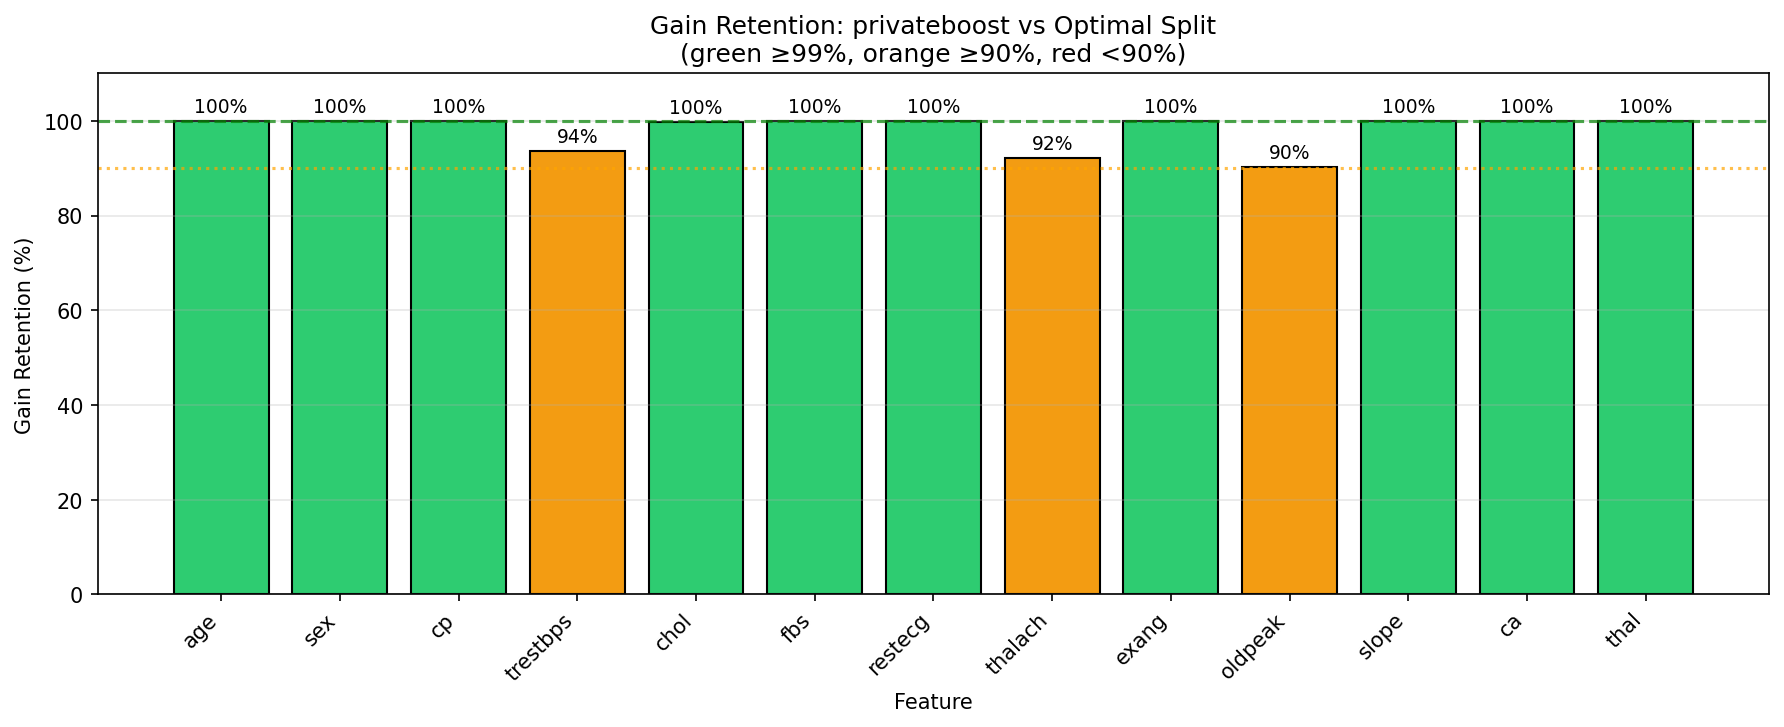
\includegraphics[width=\columnwidth]{figures/gain_retention.png}
  \caption{Split gain retention $R_f$ per feature on Heart Disease. Mean retention $\bar{R} = 98\%$ across 13 features.}
  \label{fig:gain_retention}
\end{figure}

On Heart Disease, mean retention is $\bar{R} = 98.1\%$ across 13 features, with 10 features achieving $R_f = 100\%$ (Figure~\ref{fig:gain_retention}). Histogram bins are constructed using aggregated statistics from the first protocol round, requiring no additional privacy cost. Features with skewed distributions may have suboptimal bin placement, with most data concentrated in a few bins. This explains the 90--93\% retention observed on features like \texttt{oldpeak}.

In cross-device settings, clients are intermittently available: mobile devices go offline, patients miss check-ins, or network connectivity fails. The protocol must tolerate such dropout without requiring all clients to participate in every round.

\begin{figure}[t]
  \centering
  
\includegraphics[width=\columnwidth]{figures/dropout_resilience.png}
  \caption{Test accuracy under varying client dropout rates.}
  \label{fig:dropout_resilience}
\end{figure}

The protocol naturally handles client dropout: the aggregator reconstructs from whichever clients participate in each round. We simulate dropout by randomly excluding a fraction of clients each training round, with independent sampling per round.

\textbf{Impact on reconstruction.} Client dropout does not affect the secret sharing reconstruction itself. Shamir reconstruction requires $m$ out of $n$ \textit{shareholder} responses, which is independent of client participation. Dropout reduces the number of shares each shareholder receives, but shareholders can still sum any subset of received shares and the aggregator can reconstruct the aggregate of participating clients. The minimum-client threshold enforced by shareholders (Section~\ref{sec:threat-model}) provides a lower bound: if fewer than the minimum number of clients participate, shareholders refuse to release sums, preventing reconstruction from insufficiently anonymized aggregates.

\textbf{Impact on model quality.} As shown in Figure~\ref{fig:dropout_resilience}, accuracy remains stable up to 80\% dropout across all datasets. At moderate dropout rates (20--50\%), the model sees different subsets of clients per round, which can act as a form of bagging and may improve generalization. Beyond 80\% dropout, accuracy degrades more sharply as gradient sums become noisy estimates computed from very few clients. The degradation is dataset-dependent: smaller datasets (Heart Disease, 297 samples) are more sensitive to extreme dropout than larger ones (Pima Diabetes, 768 samples).

\section{Future Work}

\subsection{Differential Privacy}

Adding calibrated Gaussian noise to gradient sums before reconstruction would provide formal $(\varepsilon, \delta)$-differential privacy~\cite{dwork2014}. Similar techniques have been applied to deep learning~\cite{abadi2016}. The noise scale can be calibrated using the mean and variance statistics already computed during the binning phase, incurring no additional privacy cost. We suggest per-tree budgets of $\varepsilon = 1.0$--$2.0$ with composition accounting across the ensemble.

\subsection{K-Anonymous Tree Structure}
\label{sec:k-anonymous}

To prevent membership inference via branch analysis, splits could be constrained to ensure at least $k$ clients in every resulting node, inspired by k-anonymity principles~\cite{sweeney2002}. This extends the existing minimum-client enforcement in shareholders to the tree structure itself. Splits that would create nodes with fewer than $k$ clients would be rejected, trading some model expressiveness for stronger privacy guarantees.

\subsection{Private Path Hiding}
\label{sec:path-hiding}

In the current protocol, the aggregator learns how many clients traverse each branch of the tree, even though it cannot identify which specific clients. This branch count information could narrow the anonymity set, particularly for branches with few clients.

A stronger privacy guarantee would hide even the branch membership. At each tree depth, clients secret-share a binary indicator for each active node: 1 if the client belongs to that node, 0 otherwise. Shareholders sum these indicators alongside the gradient shares. The aggregator reconstructs only the total count per node, learning nothing about individual assignments beyond what the count reveals.

This extension incurs communication overhead of $O(2^d \times n \times c)$ shares per gradient round, where $d$ is tree depth, $n$ is shareholders, and $c$ is clients. For $d = 3$, $n = 3$, and $c = 200$:

\begin{itemize}
  \item Current protocol: $200 \times 3 = 600$ shares per round
  \item With path hiding: $8 \times 200 \times 3 = 4{,}800$ shares per round
\end{itemize}

This $8\times$ overhead grows exponentially with depth, making the extension most practical for shallow trees ($d \leq 3$), which are common in gradient boosting. For applications with stringent privacy requirements, this tradeoff may be acceptable.

\section{Conclusion}

We presented \textit{privateboost}, a privacy-preserving federated XGBoost system for the extreme non-IID setting where each client holds only a few samples, often just one. Our protocol ensures raw data never leaves the client, requires no client-to-client coordination, and provides resilience to participant dropout.

Evaluation on medical datasets demonstrates 98\% split gain retention with accuracy comparable to centralized XGBoost. The system enables true cross-device medical federated learning where patients can participate directly without institutional intermediaries.

\section*{Acknowledgement}
The authors would like to thank the Ministry of the Economy in Luxembourg and its digital health directorate for co-supporting this research. Similarly, we would like to thank the Luxembourg National Research Fund (FNR) for partially funding this research.

\section*{Funding}
This work was supported in part by a PhD grant from the Luxembourg National Research Fund (FNR) under the project reference 17223919/MMS/Industrial Fellowship, and in part by the R-MMS clinical trial.

\bibliographystyle{unsrtnat}
\bibliography{references}

\end{document}
